\documentclass[a4paper,11pt, titlepage]{article}

\usepackage[czech]{babel}
\usepackage[IL2]{fontenc}
\usepackage[utf8]{inputenc}
\usepackage{times}
\usepackage[ruled,czech,linesnumbered,longend,noline]{algorithm2e}
\usepackage{algorithmic}
\usepackage{array,multirow}
\usepackage{graphics}
\usepackage{hyperref}
\usepackage{pdflscape}
\usepackage{tikz}

\usepackage[left=20mm, text={170mm, 240mm}, top=30mm]{geometry}

\begin{document}

\begin{titlepage}

\begin{center}
    {\Huge\textsc{Vysoké učení technické v~Brně}}\\
        \medskip
    {\huge\textsc{Fakulta informačních technologií}}\\
    \vspace{\stretch{0.382}}
    {\LARGE Typografie a~publikování\,--\,3.\,projekt}\\
        \medskip
    {\Huge Tabulky a~obrázky}\\
    \vspace{\stretch{0.618}}
\end{center}

{\LARGE \today \hfill
Róbert Ďurovič}

\end{titlepage}


\section{Úvodní strana}
Název práce umístěte do zlatého řezu a~nezapomeňte uvést dnešní datum a~vaše jméno a~příjmení.

\section{Tabulky}
Pro sázení tabulek můžeme použít buď prostředí \ \texttt{tabbing} \ nebo prostředí \ \texttt{tabular}.

\subsection{Prostředí \ \texttt{tabbing}}
Při použití \ \texttt{tabbing} \ vypadá tabulka následovně:

\begin{tabbing}
Vodní melouny \quad\= \textbf{Cena} \quad\= \textbf{Množství} \kill
\textbf{Ovoce} \> \textbf{Cena} \> \textbf{Množství}\\
Jablka \> 25,90 \> 3\,kg\\
Hrušky \> 27,40 \> 2,5\,kg\\
Vodní melouny \> 35,-- \> 1\,kus
\end{tabbing}

\bigskip

\noindent
Toto prostředí se dá také použít pro sázení algoritmů, ovšem vhodnější je použít
prostředí \ \texttt{algorithm} \ nebo \ \texttt{algorithm2e} \ (viz sekce \ref{Algoritmy}).

\subsection{Prostředí \texttt{tabular}}
Další možností, jak vytvořit tabulku, je použít prostředí \ \texttt{tabular}. Tabulky pak budou vypadat asi takto \footnote{Kdyby byl problém s \texttt{ cline,} zkuste se podívat třeba sem: \href{http://www.abclinuxu.cz/tex/poradna/show/325037}{http://www.abclinuxu.cz/tex/poradna/show/325037.}}:

\bigskip

\begin{table}[h]
\begin{center}
\catcode`\-=12 
\begin{tabular}{|c|r|r|} \hline
    & \multicolumn{2}{|c|}{\textbf{Cena}}\\\cline{2-3}
    \textbf{Měna} & \textbf{nákup} & \textbf{prodej}\\ \hline
    EUR & 27,02 & 27,20\\
    GBP & 31,08 & 31,80\\
    USD & 25,15 & 25,51\\ \hline
\end{tabular}
\caption{Tabulka kurzů k~dnešnímu dni}
\label{KurzTab}
\end{center}
\end{table}

\bigskip

\begin{table}[ht]
\catcode`\-=12
\begin{center}
\begin{tabular}{| c | c |} \hline
$A$ & $\neg A$\\ \hline
\textbf{P} & N\\ \hline
\textbf{O} & O\\ \hline
\textbf{X} & X\\ \hline
\textbf{N} & P\\ \hline
\end{tabular}
\begin{tabular}{| c | c | c | c | c | c |} \hline
\multicolumn{2}{| c |}{\multirow{2}{*}{$A \wedge B$}} & \multicolumn{4}{| c |}{$B$}\\ \cline{3-6}
\multicolumn{2}{| c |}{} & \textbf{P} & \textbf{O} & \textbf{X} & \textbf{N}\\ \hline
\multirow{4}{*}{$A$}
& \textbf{P} & P & O & X & N\\ \cline{2-6}
& \textbf{O} & O & O & N & N\\ \cline{2-6}
& \textbf{X} & X & N & X & N\\ \cline{2-6}
& \textbf{N} & N & N & N & N\\ \hline
\end{tabular}
\begin{tabular}{| c | c | c | c | c | c |} \hline
\multicolumn{2}{| c |}{\multirow{2}{*}{$A \vee B$}} & \multicolumn{4}{| c |}{$B$}\\ \cline{3-6}
\multicolumn{2}{| c |}{} & \textbf{P} & \textbf{O} & \textbf{X} & \textbf{N}\\ \hline
\multirow{4}{*}{$A$}
& \textbf{P} & P & P & P & P\\ \cline{2-6}
& \textbf{O} & P & O & P & O\\ \cline{2-6}
& \textbf{X} & P & P & X & X\\ \cline{2-6}
& \textbf{N} & P & O & X & N\\ \hline
\end{tabular}
\begin{tabular}{| c | c | c | c | c | c |} \hline
\multicolumn{2}{| c |}{\multirow{2}{*}{$A \rightarrow B$}} & \multicolumn{4}{| c |}{$B$}\\ \cline{3-6}
\multicolumn{2}{| c |}{} & \textbf{P} & \textbf{O} & \textbf{X} & \textbf{N}\\ \hline
\multirow{4}{*}{$A$}
& \textbf{P} & P & O & X & N\\ \cline{2-6}
& \textbf{O} & P & O & P & O\\ \cline{2-6}
& \textbf{X} & P & P & X & X\\ \cline{2-6}
& \textbf{N} & P & P & P & P\\ \hline
\end{tabular}
\caption{Protože Kleeneho trojhodnotová logika už je \uv{zastaralá}, uvádíme si zde příklad čtyřhodnotové logiky}
\label{Ltabs}
\end{center}
\end{table}

\section{Algoritmy}
\label{Algoritmy}

Pokud budeme chtít vysázet algoritmus, můžeme použít prostředí \  \texttt{algorithm}\footnote{Pro nápovědu jak zacházet s prostředím \ \texttt{algorithm}, můžeme zkusit tuhle stránku:\\ \href{http://ftp.cstug.cz/pub/tex/CTAN/macros/latex/contrib/algorithms/algorithms.pdf}{http://ftp.cstug.cz/pub/tex/CTAN/macros/latex/contrib/algorithms/algorithms.pdf.}} \ nebo \ \texttt{algorithm2e}\footnote{Pro \ \texttt{algorithm2e} \ zase tuhle: \href{http://ftp.cstug.cz/pub/tex/CTAN/macros/latex/contrib/algorithm2e/doc/algorithm2e.pdf}{http://ftp.cstug.cz/pub/tex/CTAN/macros/latex/contrib/algorithm2e/doc/algorithm2e.pdf.}}. Příklad použití prostředí \  \texttt{algorithm2e} \ viz Algoritmus \ref{Algoritmus}.

\bigskip

\begin{algorithm}[H]
\label{Algoritmus}
\SetNlSty{}{}{:}
\SetKwFor{For}{for}{do}{end for}
\SetKw{KwRet}{return}
\SetInd{8mm}{0cm}
\SetNlSkip{-0.43cm}
\caption{\textsc{FastSLAM}}
\KwIn{$(X_{t-1}, u_t, z_t)$}
\KwOut{\(X_{t}\)}
\BlankLine
\Indp
$\overline{X_t} = X_t = 0$\\
\For {$k =1$ to $M$}{
$x^{[k]}_t= sample\_motion\_model(u_t,x^{[k]}_{t-1})$ \\
$\omega _t^{[k]}=measurement\_model(z_t,x_t^{[k]},m_{t-1})$ \\
$m_t^{[k]}=updated\_occupancy\_grid(z_t,x_t^{[k]},m^{[k]}_{t-1})$\\
$\overline{X_t} = \overline{X_t} + \langle x_x^{[m]},\omega ^{[m]}_t\rangle$}{}
\For {$k =1$ to $M$}{
draw $i$ with probability $\approx \omega^{[i]}_{t}$  \\
add $ \langle x^{[k]}_{x}$ , $m_{t}^{[k]}\rangle$ to $X_t$}{}
\KwRet{\(X_{t}\)}
\end{algorithm}

\bigskip

\section{Obrázky}
Do našich článků můžeme samozřejmě vkládat obrázky. Pokud je obrázkem fotografie, můžeme klidně použít bitmapový soubor. Pokud by to ale mělo být nějaké schéma nebo něco podobného, je dobrým zvykem takovýto obrázek vytvořit vektorově.
\begin{figure}[ht]
\begin{center}
	\scalebox{0.4}{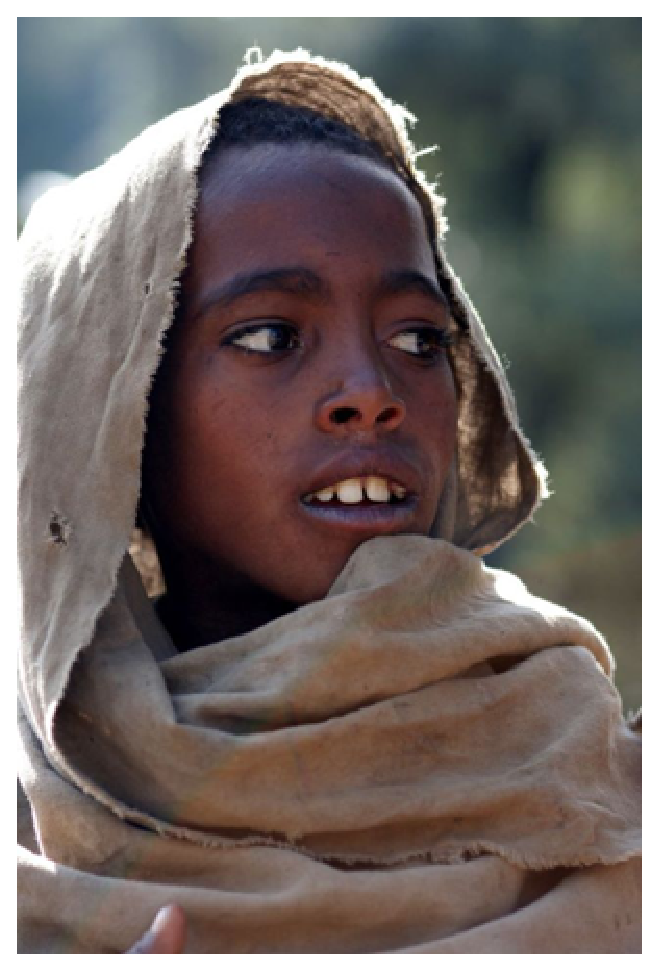
\includegraphics{etiopan.eps}
	\hspace{-2mm}
	\reflectbox{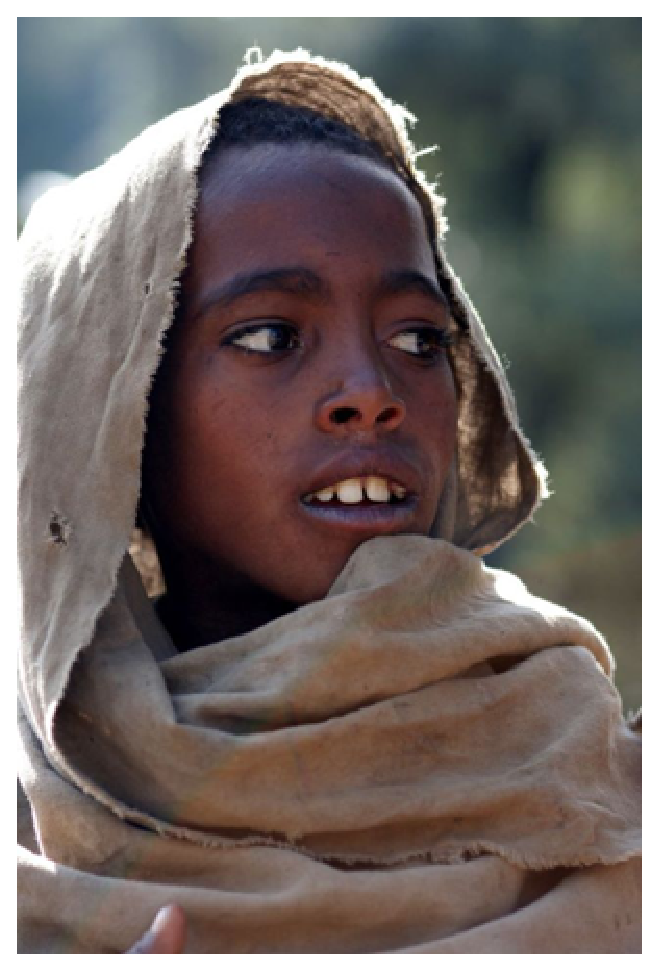
\includegraphics{etiopan.eps}} }
	\caption{Malý etiopánek a~jeho bratříček}
	\label{img1}
\end{center}
\end{figure}

\newpage

Rozdíl mezi vektorovým\, \ldots
\begin{figure}[ht]
\begin{center}
    \scalebox{0.4}{
\includegraphics{oniisan.eps}}
    \caption{Vektorový obrázek}
    \label{img2}
\end{center}
\end{figure}

\noindent \ldots\,a~bitmapovým obrázkem
\begin{figure}[ht]
\begin{center}
    \scalebox{0.59}{
\includegraphics{oniisan2.eps}}
    \caption{Bitmapový obrázek}
    \label{img3}
\end{center}
se projeví například při zvětšení.

\quad Odkazy (nejen ty) na obrázky \ref{img1}, \ref{img2} a~\ref{img3}, na tabulky \ref{KurzTab} a \ref{Ltabs} a~také na algoritmus \ref{Algoritmus} jsou udělány pomocí křížových odkazů. Pak je ovšem potřeba zdrojový soubor přeložit dvakrát.

\quad Vektorové obrázky lze vytvořit i~přímo v \LaTeX u, například pomocí prostředí \ \texttt{picture}.
\end{figure}

\newpage

\begin{landscape}
\begin{picture}(0,330)
\put(3,1){\linethickness{1mm}\framebox(670,290){
\begin{tikzpicture}[y=0.59pt, x=0.59pt, yscale=-1.000000, xscale=1.000000, inner sep=0pt, outer sep=0pt]
\path[draw=black,line join=miter,line cap=butt,miter limit=4.00,line
  width=4.261pt] (-1.0427,282.6131) .. controls (1129.9598,284.6472) and
  (1018.6767,281.4023) .. (1018.6767,281.4023);
\path[draw=black,line join=miter,line cap=butt,line width=0.800pt]
  (173.7226,279.2774) .. controls (175.1825,210.6642) and (175.1825,210.6642) ..
  (175.1825,210.6642) .. controls (356.9343,210.6642) and (356.9343,210.6642) ..
  (356.9343,210.6642) .. controls (516.7883,275.6277) and (516.0584,276.3577) ..
  (516.0584,276.3577);
\path[draw=black,line join=miter,line cap=butt,line width=0.800pt]
  (119.7080,278.5475) .. controls (122.6277,101.9051) and (122.6277,101.9051) ..
  (122.6277,101.9051) .. controls (336.4964,104.0949) and (336.4964,104.0949) ..
  (336.4964,104.0949);
\path[draw=black,line join=miter,line cap=butt,line width=0.800pt]
  (911.6788,166.1387) .. controls (911.6788,166.1387) and (911.6788,166.1387) ..
  (213.1387,159.5693) .. controls (213.1387,159.5693) and (213.1387,159.5693) ..
  (213.8686,129.6423) .. controls (911.6788,130.3723) and (911.6788,130.3723) ..
  (911.6788,130.3723);
\path[draw=black,line join=miter,line cap=butt,line width=0.800pt]
  (335.7664,128.1825) .. controls (336.4964,79.2774) and (336.4964,79.2774) ..
  (336.4964,79.2774) .. controls (615.3285,80.7372) and (616.7883,80.7372) ..
  (616.7883,80.7372) .. controls (616.0584,124.5328) and (616.0584,125.2628) ..
  (616.0584,125.2628);
\path[draw=black,line join=miter,line cap=butt,line width=0.800pt]
  (616.7883,115.0438) .. controls (858.3942,117.9635) and (858.3942,117.9635) ..
  (858.3942,117.9635) .. controls (857.6642,128.9124) and (857.6642,128.9124) ..
  (857.6642,128.9124);
\path[draw=black,line join=miter,line cap=butt,line width=0.800pt]
  (423.3577,237.6715) .. controls (910.9489,238.4015) and (910.9489,238.4015) ..
  (910.9489,238.4015) .. controls (911.6788,280.7372) and (911.6788,280.7372) ..
  (911.6788,280.7372);
\path[draw=black,line join=miter,line cap=butt,miter limit=4.00,line
  width=1.600pt] (900.0000,169.0584) .. controls (900.7299,234.7518) and
  (900.7299,234.7518) .. (900.7299,234.7518);
\path[draw=black,line join=miter,line cap=butt,miter limit=4.00,line
  width=0.800pt] (214.5985,161.0292) .. controls (271.5328,210.6642) and
  (272.2628,210.6642) .. (272.2628,210.6642);
\path[draw=black,line join=miter,line cap=butt,miter limit=4.00,line
  width=1.600pt] (910.9489,165.4088) .. controls (910.2190,130.3723) and
  (910.9489,130.3723) .. (910.9489,130.3723);
\path[draw=black,line join=miter,line cap=butt,line width=0.800pt]
  (375.9124,216.5036) .. controls (375.9124,166.8686) and (375.9124,166.8686) ..
  (375.9124,166.8686);
\path[draw=black,line join=miter,line cap=butt,line width=0.800pt]
  (375.9124,167.5985) .. controls (899.2701,171.2482) and (898.5402,171.2482) ..
  (898.5402,171.2482);

\end{tikzpicture}
}}
\end{picture}
\end{landscape}

\end{document}
